\documentclass[11pt]{article}

% load packages and functions
%%%%%%%%%%%%%%%%
% Header for attribution
%%%%%%%%%%%%%%%%

%\pagestyle{fancy}
%
%\fancyhead{}
%
%\renewcommand{\headrulewidth}{0.25pt}
%\renewcommand{\footrulewidth}{0pt}
%\headsep = 30pt 
%\footskip = 30pt
%
%\chead{{\footnotesize Derivative of \href{http://www.opeintro.org}{\textit{OpenIntro}} project}}

%%%%%%%%%%%%%%%%
% Packages
%%%%%%%%%%%%%%%%

\usepackage[sc]{mathpazo}
%\usepackage[T1]{fontenc}
\usepackage{geometry}
\geometry{verbose,tmargin=2cm,bmargin=2.2cm,lmargin=2.5cm,rmargin=2.5cm}
\setcounter{secnumdepth}{2}
\setcounter{tocdepth}{2}
\usepackage{url}
\usepackage{xcolor}
\usepackage[parfill]{parskip}
\usepackage{graphicx}
\usepackage{amssymb}
\usepackage{amsmath}
\usepackage{epstopdf}
\usepackage{enumerate}
\usepackage{colortbl}
\usepackage{xcolor}
\usepackage{sectsty}
\usepackage{multicol}
\usepackage{fancyhdr}
\usepackage{changepage}
\usepackage{textcomp}
\usepackage{endnotes}
\usepackage{breakurl}

%%%%%%%%%%%%%%%%
% Colors and hyperref
%%%%%%%%%%%%%%%%

\definecolor{oiB}{rgb}{.337,.608,.741}
\definecolor{oiR}{rgb}{.941,.318,.200}
\definecolor{oiG}{rgb}{.298,.447,.114}
\definecolor{oiY}{rgb}{.957,.863,0}

\usepackage[unicode=true, pdfusetitle, bookmarks=true, bookmarksnumbered=true, bookmarksopen=true, bookmarksopenlevel=2, breaklinks=false, pdfborder={0 0 1}, backref=false, colorlinks=true, linkcolor = oiB, urlcolor= oiB]{hyperref}
\hypersetup{pdfstartview={XYZ null null 1}}

%%%%%%%%%%%%%%%%%
%% Color section headings
%%%%%%%%%%%%%%%%%

\allsectionsfont{\color{oiB}}              
 
%%%%%%%%%%%%%%%%
% Exercise environment
%%%%%%%%%%%%%%%%

\newenvironment{exercise}
{
\addvspace{5mm}
\begin{adjustwidth}{0em}{3em}
\begin{itemize}\item[]\refstepcounter{equation}\noindent\normalsize\textbf{\textcolor{oiB}{Exercise \theexercise}}
}
{\normalsize

\addvspace{3mm}
\end{itemize}
\end{adjustwidth}
}

\newcommand\theexercise{\arabic{equation}}

%%%%%%%%%%%%%%%%
% Menu items
%%%%%%%%%%%%%%%%

\newcommand{\menu}[1]{\textsf{#1}}

%%%%%%%%%%%%%%%%
% Formatted url
%%%%%%%%%%%%%%%%

\newcommand{\web}[1]{\urlstyle{same}\textit{\url{#1}}}

%%%%%%%%%%%%%%%%
% Footnote using symbols
% 1 - *
% 2 - dagger
% 3 - double dagger
% 4 - ... 9 (see page 175 of the latex manual)
% http://help-csli.stanford.edu/tex/latex-footnotes.shtml
%%%%%%%%%%%%%%%%

\long\def\symbolfootnote[#1]#2{\begingroup%
\def\thefootnote{\fnsymbol{footnote}}\footnote[#1]{#2}\endgroup}

%%%%%%%%%%%%%%%%
% Non-numbered footnote for license and attribution
%%%%%%%%%%%%%%%%

\newcommand{\license}[1]{\let\thefootnote\relax\footnotetext{#1}}

%%%%%%%%%%%%%%%%
% Set padding in code chunk boxes
%%%%%%%%%%%%%%%%

\setlength\fboxsep{2mm}

%%%%%%%%%%%%%%%%
% Place spacing between text and code chunk boxes
%%%%%%%%%%%%%%%%

\ifdefined\knitrout
  \renewenvironment{knitrout}{
    \vspace{1em}
  }{
    \vspace{1em}
  }
\else
\fi

%%%%%%%%%%%%%%%%
% Redefine inline code commands to change the font to texttt
%%%%%%%%%%%%%%%%

\renewcommand{\hlfunctioncall}[1]{\textcolor[rgb]{0.11,0.53,0.93}{\texttt{#1}}}%

\renewcommand{\hlstring}[1]{\textcolor[rgb]{0.65,0.50,0.39}{\texttt{#1}}}%

\renewcommand{\hlsymbol}[1]{\textcolor[rgb]{0.387,0.581,0.148}{\texttt{#1}}}%

\renewcommand{\hlkeyword}[1]{\textcolor[rgb]{0.31,0.65,0.76}{\texttt{#1}}}%

\renewcommand{\hlargument}[1]{\textcolor[rgb]{0.31,0.41,0.53}{\texttt{#1}}}%

\renewcommand{\hlnumber}[1]{\textcolor[rgb]{0.387,0.581,0.148}{\texttt{#1}}}%



%\newcommand{\soln}[1]{\textcolor{purple}{\textit{#1}}}		% For showing solutions
\newcommand{\soln}[1]{ }	% For hiding solutions

\newcommand{\note}[1]{\textcolor{red}{\textit{#1}}}

% document
\begin{document}

\section*{Lab 8: Multiple regression}

\subsection*{LA Housing Data}
\begin{quote}
``Transparency is a core value at Google. As a company we feel it is our responsibility to ensure that we maximize transparency around the flow of information related to our tools and services. We believe that more information means more choice, more freedom and ultimately more power for the individual.''
\end{quote}

So begins Google's recently released Transparency Report.  As a company, they have access to prodigious amounts of information about their users, information that is often of keen interest to governments.  The report contains information related to the number of government inquiries for user data as well as the number of requests to remove content from Google's services. In this lab we'll consider a handful of countries and various statistics on each to help us get a sense of what defines countries with various levels of internet censorship.  Our tool of choice here will be multiple linear regression, and while it might not be the method best suited to this particular situation, it can still provide us with useful insights.

\subsection*{The data}

The data consist of the number of requests Google received for user account information as part of criminal investigations in the first half of 2011 and the rate of compliance as well as some other indicators on the countries.

Let's load up the Google data:

\begin{lstlisting}
download.file("http://stat.duke.edu/courses/Fall11/sta101.02/labs/goog.csv", destfile = "goog.csv")
\end{lstlisting}

Below is a list of the variables and descriptions.

\begin{table}[h] \small
\begin{tabular}{r | p{14cm}}
\code{city} 		& name of country. \\
\code{type} 	& percentage of requests Google complied with. \\
\code{bed}	& number of requests Google received for user account information as part of criminal investigations. \\
\code{bath} 		& population of country, in thousands. \\
\code{garage} 		& human development index, a composite measure of life expectancy, literacy, education, and standard of living categorized into \code{sqrt} democracies, \code{flawed} democracies, and \code{hybrid regimes}. For more information, click \href{http://en.wikipedia.org/wiki/List_of_countries_by_Human_Development_Index}{here}. \\
\code{sqft} 		& democracy index, measured on a scale of zero to ten (full democracy). For more information, click \href{http://en.wikipedia.org/wiki/Democracy_Index}{here}. \\
%\code{dem_cat} 	& categorical variable for democracy index. \\
\code{pool} 		& percentage of internet users. For more information, click \href{http://en.wikipedia.org/wiki/List_of_Internet_users_by_country}{here}. \\
%\code{freepress} 	& freedom of press index. \note{add link} \\
\code{price} 	& free press index, scored on a scale from 1 (most free) to 100 (least free). For more information, click \href{http://en.wikipedia.org/wiki/Freedom_of_the_Press_(report)}{here}. \\
\end{tabular}
\end{table}

We'll first focus on modeling Google's compliance rate (\code{complied}) using the rest of the explanatory variables.

\subsection*{Pairwise plots}

We start our analysis by examining pairwise plots of the data. Since the first column is just the country name, we leave that column out. 

\begin{lstlisting}
plot(goog[,-1])
\end{lstlisting}

Note that you could also get the same plot with \code{plot(goog[,2:8])} but it's a bit quicker to use \code{[,-1]}, saying that you want all columns except for the first one.

\begin{exercise}
Examine the pairwise scatterplots. What can you say about the trends in relationships between \code{complied} and the other variables? Are there any observations that stand out from the rest?
\end{exercise}
\soln{None of the variables seem to have a particularly linear relationship with \% complied. Perhaps the strongest linear relationship is between \% complied and HDI. There appears to be at least one outlier, the country with the highest population.}

\subsection*{Drop outliers}

One of the observations that stands out as unusual is the country with the highest population. Let's see which country this is:

\begin{lstlisting}
which.max(goog$pop)
\end{lstlisting}

The result of the above function indicates that the observation in the 10th row of the data set is the country with the highest population, and this country is India. Next, we subset the data to exclude this observation.

\begin{lstlisting}
goog_sub = subset(goog, country != "india")
\end{lstlisting}

Let's take another look at the pairwise plots.

\begin{lstlisting}
plot(goog_sub[,-1])
\end{lstlisting}

\begin{exercise}
Do any other countries appear unusual in this plot? If so, determine which one(s).
\end{exercise}
\soln{The country with the highest number of requests (US) appears unusual.}
%\begin{lstlisting}
%which.max(goog_sub$requests)
%\end{lstlisting}

Regardless of your answer, we'll proceed with the analysis with the 25 countries remaining in the data frame \code{goog_sub}.

\subsection*{Defining the reference level}

Currently there is one categorical variable in the data, \code{dem}. Let's make a frequency table for this variable.

\begin{lstlisting}
table(goog_sub$dem)
\end{lstlisting}

The level that shows up first, \code{free}, is by default the reference level. R usually chooses the reference level as the level that comes up first alphabetically. We can change the reference level to \code{hybrid} using the following command:

\begin{lstlisting}
goog_sub$dem = relevel(goog_sub$dem, ref = "hybrid")
\end{lstlisting}

\begin{exercise}
Confirm that the reference level for \code{dem} has been changed to \code{hybrid}.
\end{exercise}
\soln{Yes, not shows up as the first level in the table.}
%\begin{lstlisting}
%table(goog_sub$dem)
%\end{lstlisting}

\subsection*{Multiple linear regression}

Let's fit a multiple linear regression model to predict compliance rate using the rest of the explanatory variables.

\begin{lstlisting}
m_full = lm(complied ~ requests + pop + hdi + dem + internet + freepress, data = goog_sub)
summary(m_full)
\end{lstlisting}

The format here is similar to what we used for simple regression, only now we have many predictors, each separated by \code{+}.

\begin{exercise}
Interpret the coefficient for \code{pop} (population) and the coefficients associated with the democracy index.
\end{exercise}
\soln{The model predicts a 1.642e-04 percent increase in Google's compliance rate for each additional thousand of population. \\
The model estimates a 1.37\% increase in compliance rate in countries with a flawed democracy, compared to those with a hybrid regime, and 1.007\% increase in compliance rate in countries with full democracy compared to those with a hybrid regime. \\
\textbf{TAs: make sure to mention that the coefficients always compare to the reference level.}}

\subsection*{Model selection}

\begin{exercise}
Which variables in the full model are significant predictors?
\end{exercise}
\soln{None of them}

Let's try to find a model that better predicts Google's compliance rate than the full model. For this we can use the \code{step} function to do a stepwise model selection. By default this function does backwards-elimination.

\begin{lstlisting}
step(m_full)
\end{lstlisting}

The second to last argument in the output shows that the formula for the best model is \code{lm(formula = complied ~ pop + hdi, data = goog_sub)}. So let's try that model and see what the output looks like.

\begin{lstlisting}
m = lm(complied ~  pop  + hdi, data = goog_sub)
summary(m)
\end{lstlisting}

\vfill

\begin{center}
\textit{On your own part on the next page.}
\end{center}

%

\pagebreak

\subsection*{On Your Own}

You should work with your teammates on the lab, as well as the homework from the book, but you must turn in your own work. The answers to questions must be in your own words.\\

\begin{enumerate}

\item Do the countries in this data set represent a population or a sample? If you answered ``sample�, then what is the population of interest? Do these countries represent a random sample from this population? Is it reasonable to assume this sample is representative of the population? Why or why not?

\item Copy and paste the R output of the final model and interpret the slope estimates of the variables. Also comment on whether or not the p-values for these coefficients are meaningful in this context. (Hint: What is the null hypothesis for testing for significance of a slope coefficient in the context of multiple linear regression? What does a p-value mean in this context?)

%\begin{lstlisting}
%Call:
%lm(formula = complied ~ pop + hdi, data = goog_sub)
%
%Residuals:
%    Min      1Q  Median      3Q     Max 
%-41.239 -13.401   2.113  10.399  48.533 
%
%Coefficients:
%              Estimate Std. Error t value Pr(>|t|)   
%(Intercept) -1.551e+02  5.794e+01  -2.678  0.01375 * 
%pop          1.290e-04  6.173e-05   2.090  0.04841 * 
%hdi          2.356e+02  6.657e+01   3.540  0.00184 **
%---
%Signif. codes:  0 '***' 0.001 '**' 0.01 '*' 0.05 '.' 0.1 ' ' 1 
%
%Residual standard error: 20.38 on 22 degrees of freedom
%Multiple R-squared: 0.393,	Adjusted R-squared: 0.3378 
%F-statistic: 7.121 on 2 and 22 DF,  p-value: 0.004123 
%\end{lstlisting}

\soln{For each additional person in the population count we would expect compliance rate to increase on average by 0.000129\%. For each additional 0.001 in HDI we would expect compliance rate to increase on average by 0.1356\%. Both variables are significant predictors.}

\item Check model diagnostics on the final model. You may want to refer to code from the previous lab to do this as well as the Section 8.3 from the book on graphical model diagnostics for multiple linear regression.

\soln{
TAs: You will likely need to help students with the code for this part, so make sure to work on it together as a class.
\begin{enumerate}[1.]
\item nearly normal residuals: the normal probability plot shows some deviance from normality but not a lot, and the histogram shows nearly normally distributed residuals.
\begin{center}
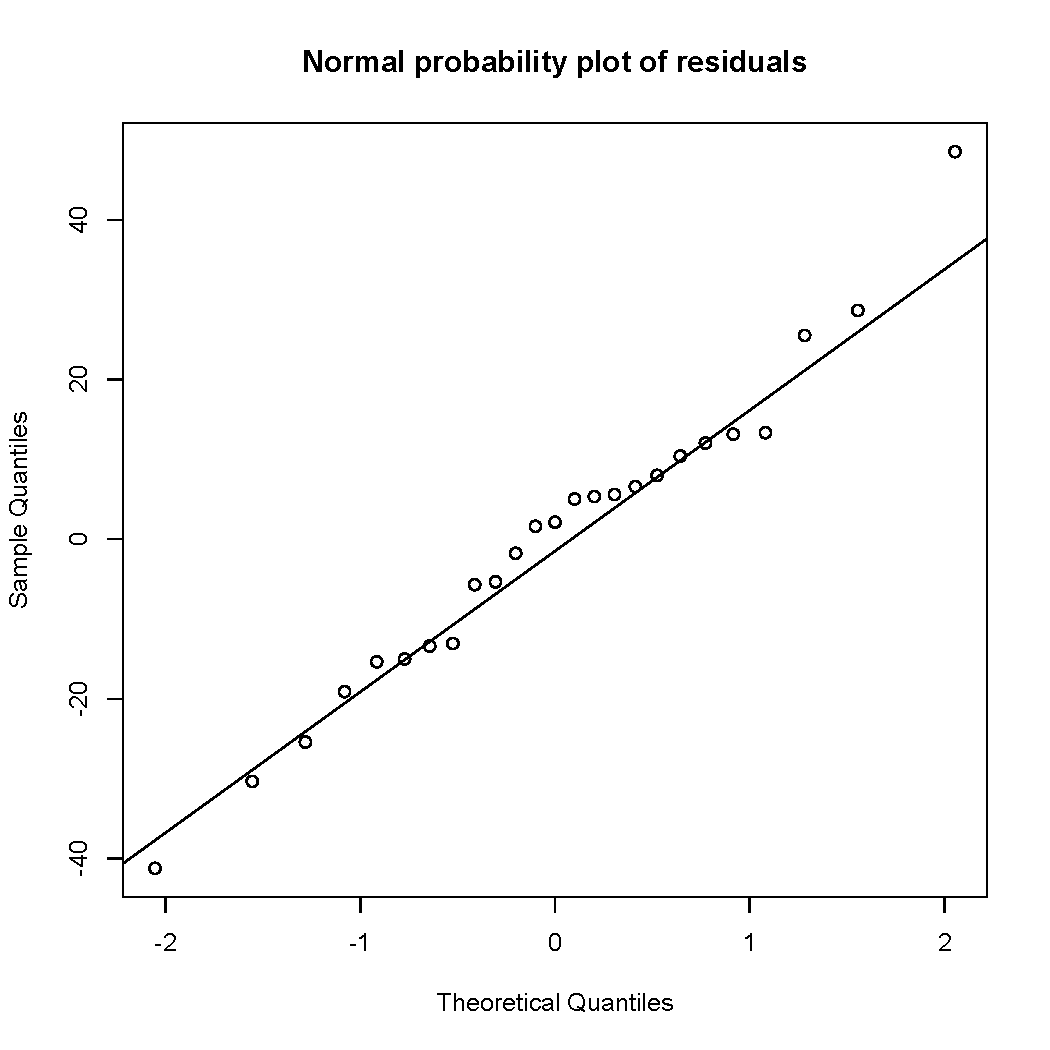
\includegraphics[width=0.4\textwidth]{figures/qqnorm_res}
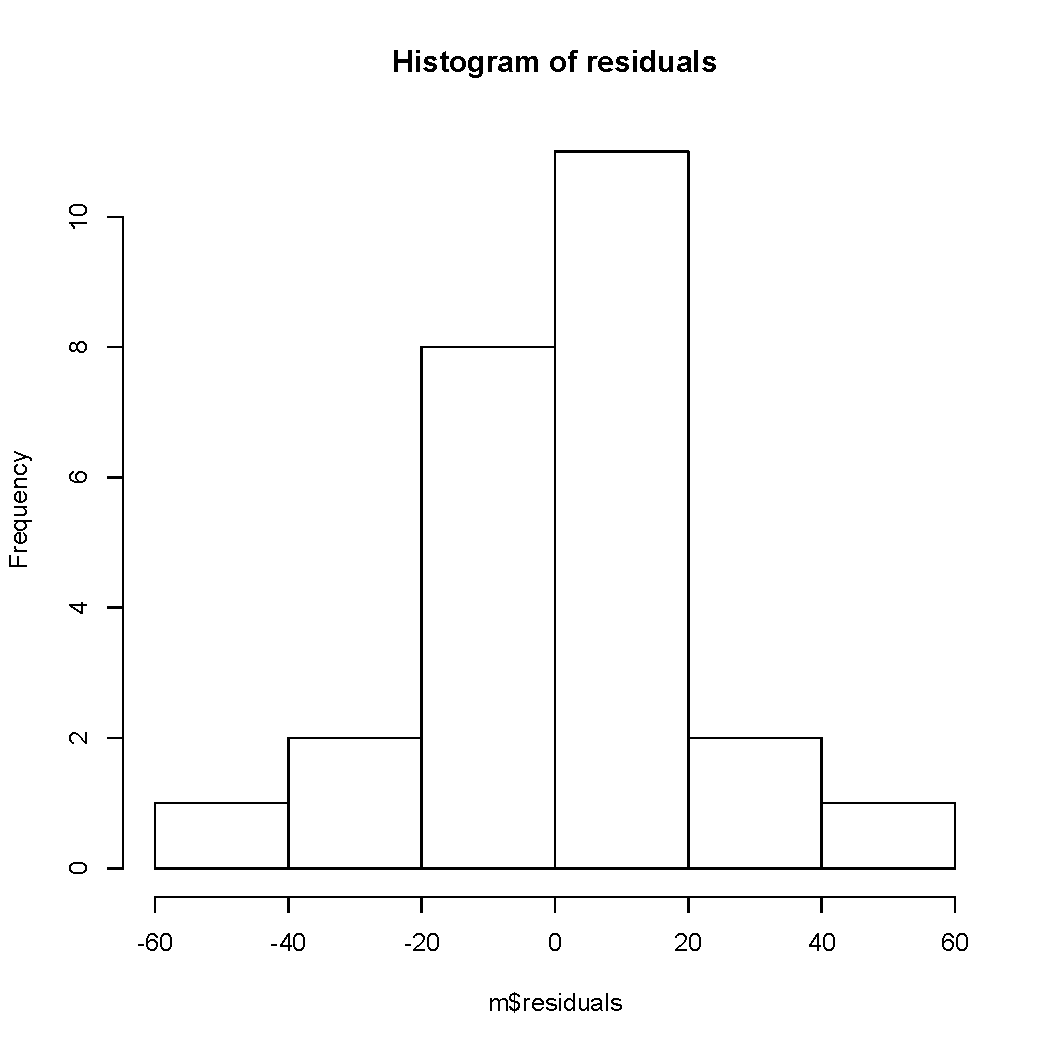
\includegraphics[width=0.4\textwidth]{figures/hist_res}
\end{center}
\item constant variance of residuals: there seems to be a fan shape in the residuals vs. fitted plot so this condition is definitely violated. students can also do a absolute value of residuals vs. fitted plot.
\begin{center}
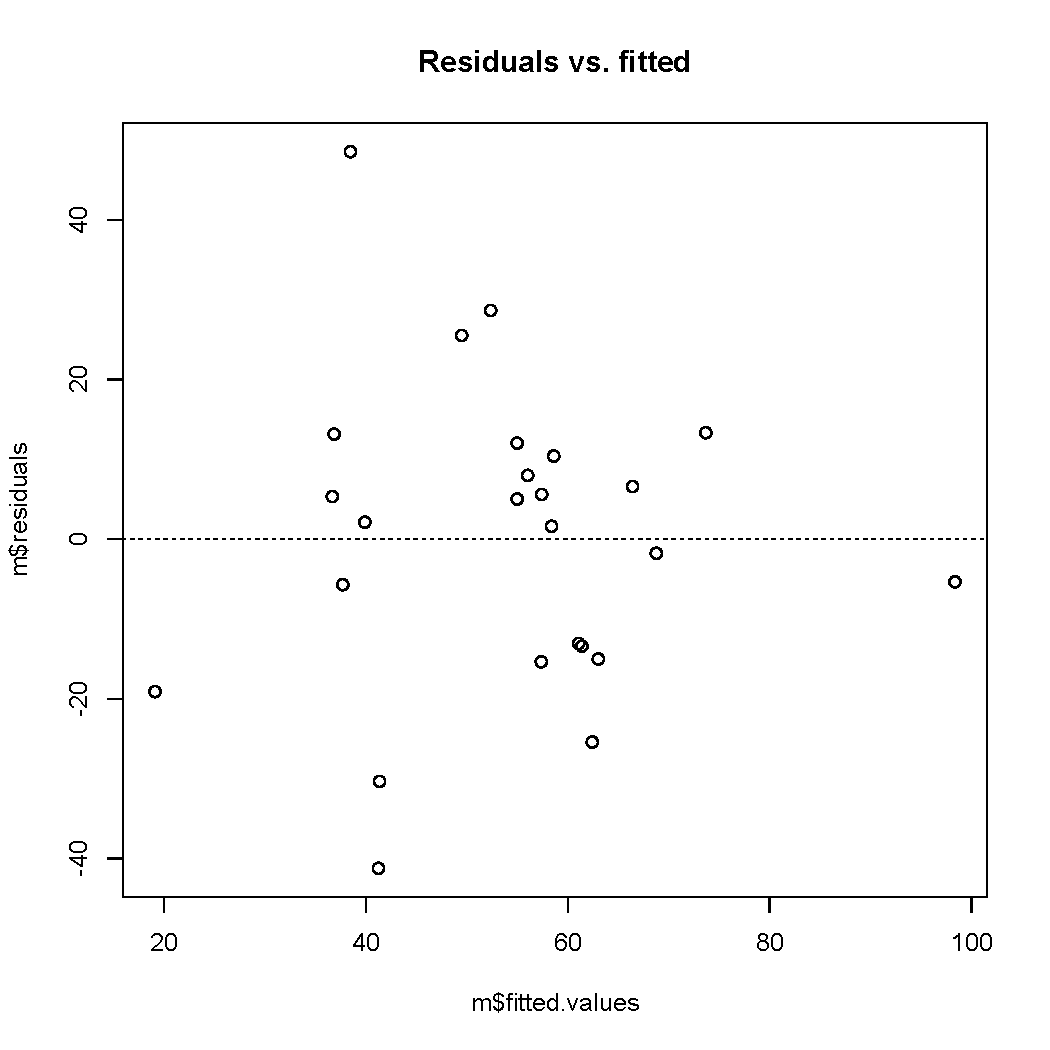
\includegraphics[width=0.4\textwidth]{figures/res_fit}
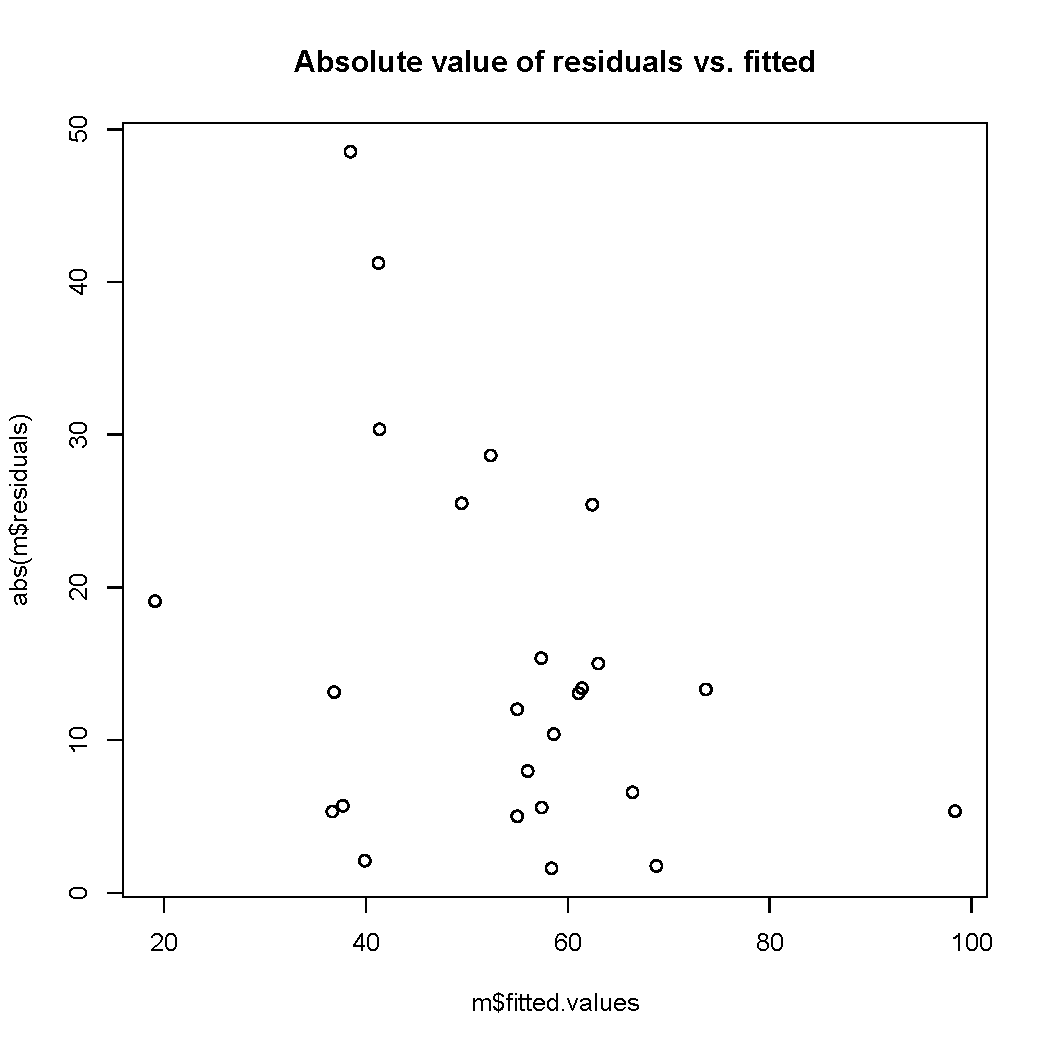
\includegraphics[width=0.4\textwidth]{figures/abs_res_fit}
\end{center}
\item independent residuals: there is no apparent increasing or decreasing trend in the residuals vs. order of data collection plot, therefore this condition is satisfied.
\begin{center}
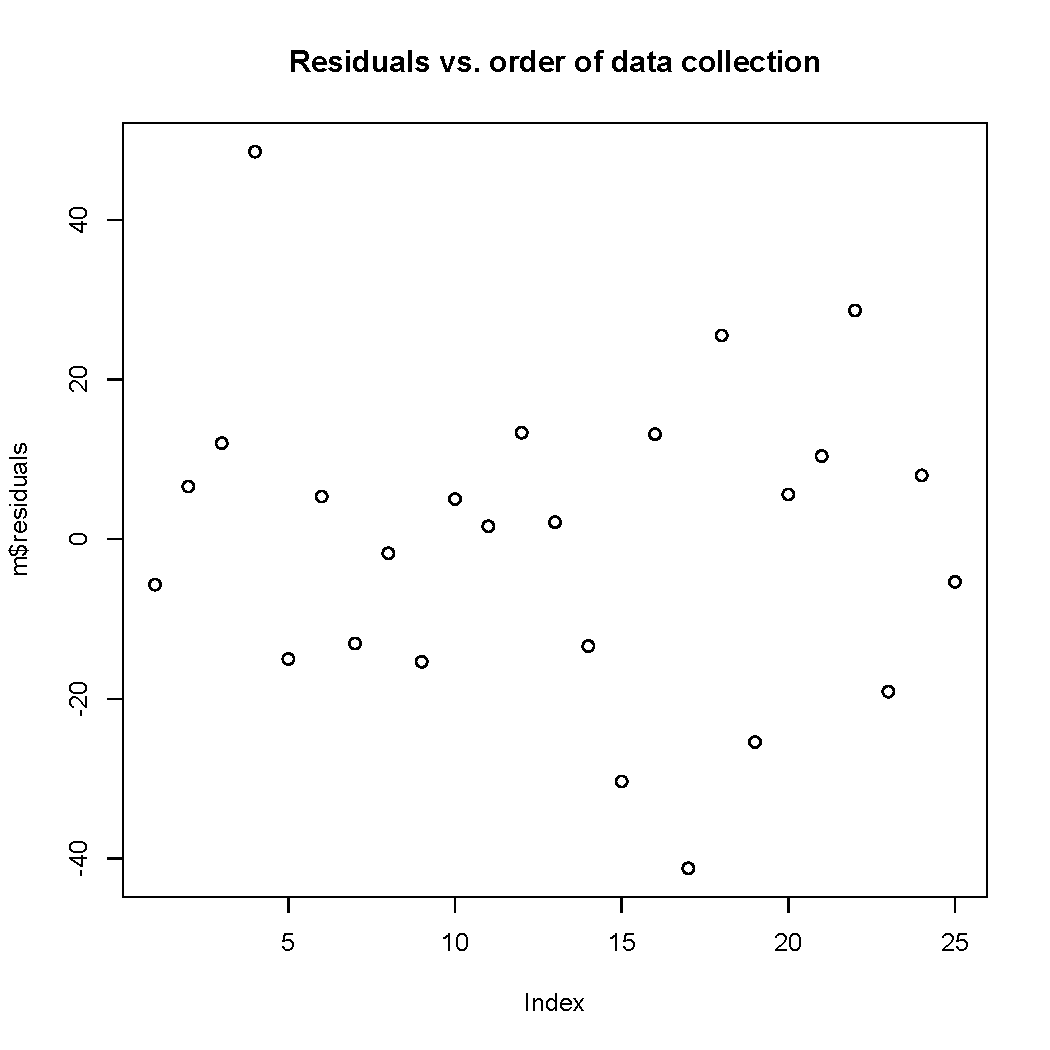
\includegraphics[width=0.4\textwidth]{figures/res_order}
\end{center}
\item each variable is linearly related to the outcome: only HDI and internet are linearly related to the outcome. we wouldn't expect to see a linear pattern in the complied vs. democracy plot since democracy index is categorical, but we should have seen linear relationships in the other plots. (students might also just provide separate plots for each relationship)
\begin{center}
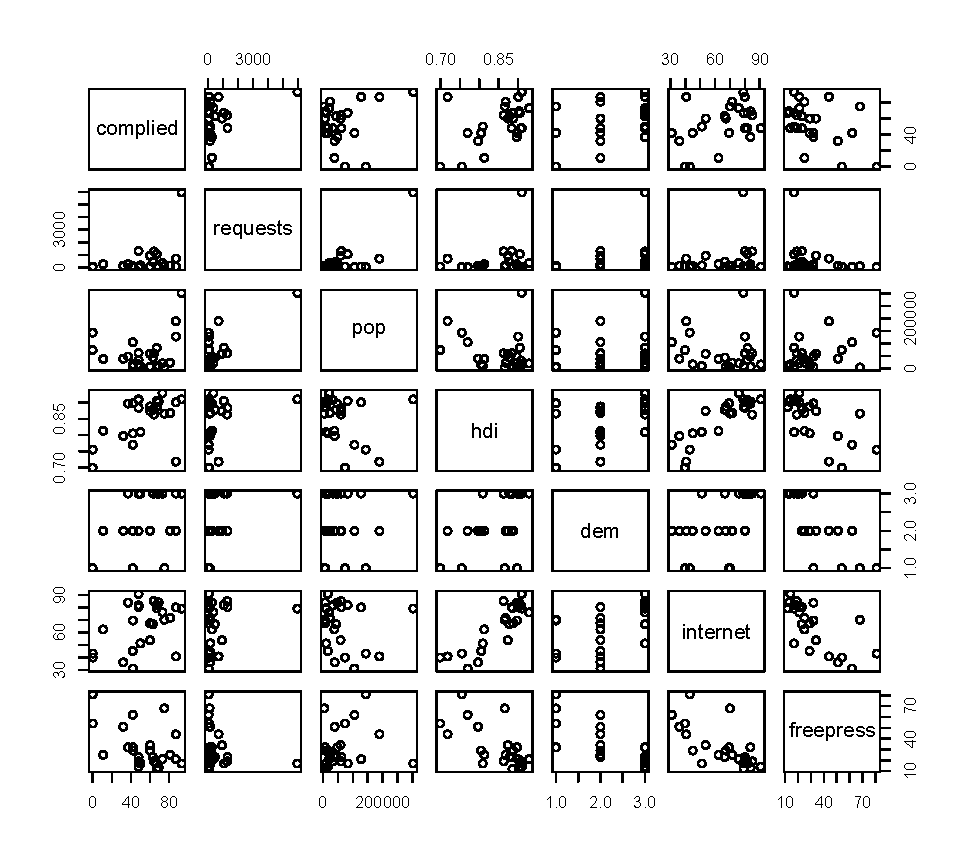
\includegraphics[width=\textwidth]{figures/pairwise}
\end{center}
\end{enumerate}
}

%\begin{lstlisting}
%# normal residuals
%qqnorm(m$residuals)
%qqline(m$residuals)
%hist(m$residuals)
%
%# constant variance residuals
%plot(m$residuals ~ m$fitted.values, main = "Residuals vs. fitted")
%abline(h = 0, lty = 3)
%
%plot(abs(m$residuals) ~ m$fitted.values, main = "Absolute value of residuals vs. fitted")
%
%# independent residuals
%plot(m$residuals, main = "Residuals vs. order of data collection")
%
%# linear relationship
%plot(goog_sub[,-1])
%\end{lstlisting}

\item Fit another model predicting number of \code{requests} from all other explanatory variables except for compliance rate. Using the \code{step()} function find the ``best" model and include only the output for this model.

%\begin{lstlisting}
%m_req_full = lm(requests ~  pop + hdi + dem + internet + freepress, data = goog_sub)
%step(m_req_full)
%m_req = lm(requests ~ pop + hdi, data = goog_sub)
%summary(m_req)
%\end{lstlisting}

%\begin{lstlisting}
%Call:
%lm(formula = requests ~ pop + hdi, data = goog_sub)
%
%Residuals:
%     Min       1Q   Median       3Q      Max 
%-1805.62  -272.53    21.02   348.95  1474.24 
%
%Coefficients:
%              Estimate Std. Error t value Pr(>|t|)    
%(Intercept) -6.785e+03  1.895e+03  -3.581  0.00167 ** 
%pop          1.445e-02  2.019e-03   7.158 3.55e-07 ***
%hdi          7.566e+03  2.177e+03   3.476  0.00215 ** 
%---
%Signif. codes:  0 '***' 0.001 '**' 0.01 '*' 0.05 '.' 0.1 ' ' 1 
%
%Residual standard error: 666.5 on 22 degrees of freedom
%Multiple R-squared: 0.7134,	Adjusted R-squared: 0.6873 
%F-statistic: 27.38 on 2 and 22 DF,  p-value: 1.073e-06 
%\end{lstlisting}

\end{enumerate}

$\:$ \\

\textit{Note that you might find that your model violates some assumptions. You might  have similar issues with models you use for your projects. Multiple linear regression, while a powerful method, is still considered basic. Lots of real data sets will require more advanced techniques for proper analysis. If you are interested in what else is out there I encourage you to take a higher level statistics course next semester/year to learn such techniques.}


\end{document}